\section{Środowisko testowe}
\label{sec:testing}
    Podczas budowy, dowolnego systemu, niezwykle ważne jest testowanie elementów składowych każdego z bloków.
    W informatyce, testowanie oprogramowania zapewniają testy jednostkowe, które sprawdzają działanie poszczególnych algorytmów i programów.
    W przypadku prac nad hardwarem, niezbędne jest zbudowanie odpowiedniego środowiska, pozwalającego na testowanie każdego elementu osobno oraz łącznie z innymi elementami.
    Dlatego pracę nad projektem można podzielić na kilka części:
    \begin{enumerate}
        \item Budowa prototypu na płytce stykowej.
        \item Złożenie ramy pojazdu, z elektroniką umieszczoną na płytce stykowej, wraz z doprowadzonym zewnętrznym zasilaniem.
        \item Sprawdzenie działania pojazdu z płytką stykową zasilaną bateryjnie.
        \item Wykonanie płytki prototypowej, z połączeniami wszystkich elementów na stałe ponownie z zewnętrznym zasilaniem.
        \item Sprawdzenie działania prototypu pojazdu z zasilaniem akumulatorowym.
    \end{enumerate}
    Każdy z wymienionych etapów charakteryzował się innym rodzajem testów oraz innymi problemami.
    A przejście z etapu do etapu, było możliwe dopiero po uznaniu przez autora, że układ pracuje poprawnie.

    \subsection{Modele prototypowe}
        Pierwszym etapem, było zbudowanie modelu elektronicznego na płytce stykowej, na podstawie schematu \ref{schema:block}.
        Poniżej przedstawiono zdjęcie układu złożonego na breadboardzie.
        Układ ten, pozwalał na bezpieczne testowanie nowych funkcji, bez ryzyka uszkodzenia elementów.
        Dodatkową zaletą tego modelu, jest możliwość debugowania kodu bezpośrednio na płytce, a nie poprzez symulację.
        \begin{figure}[!ht]
            \centering
            \includegraphics[width = 0.7\textwidth, trim = {500px, 500px, 350px, 350px}, clip]{Breadboard.jpg}
            \caption{Model prototypowy na płytce stykowej}
            \label{fig:breadboard}
        \end{figure}

        Zbudowany model z płytki stykowej, został skompresowany aby zmieścił się na pojedynczej płytce o rozmiarach 400-stu pól.
        Tak ściśnięty układ można było założyć na ramę pojazdu.
        W tym celu została zaprojektowana i wydrukowana mała podpora, która pozwoliła na sztywne zamocowanie układu.

        \begin{figure}[!ht]
            \centering
            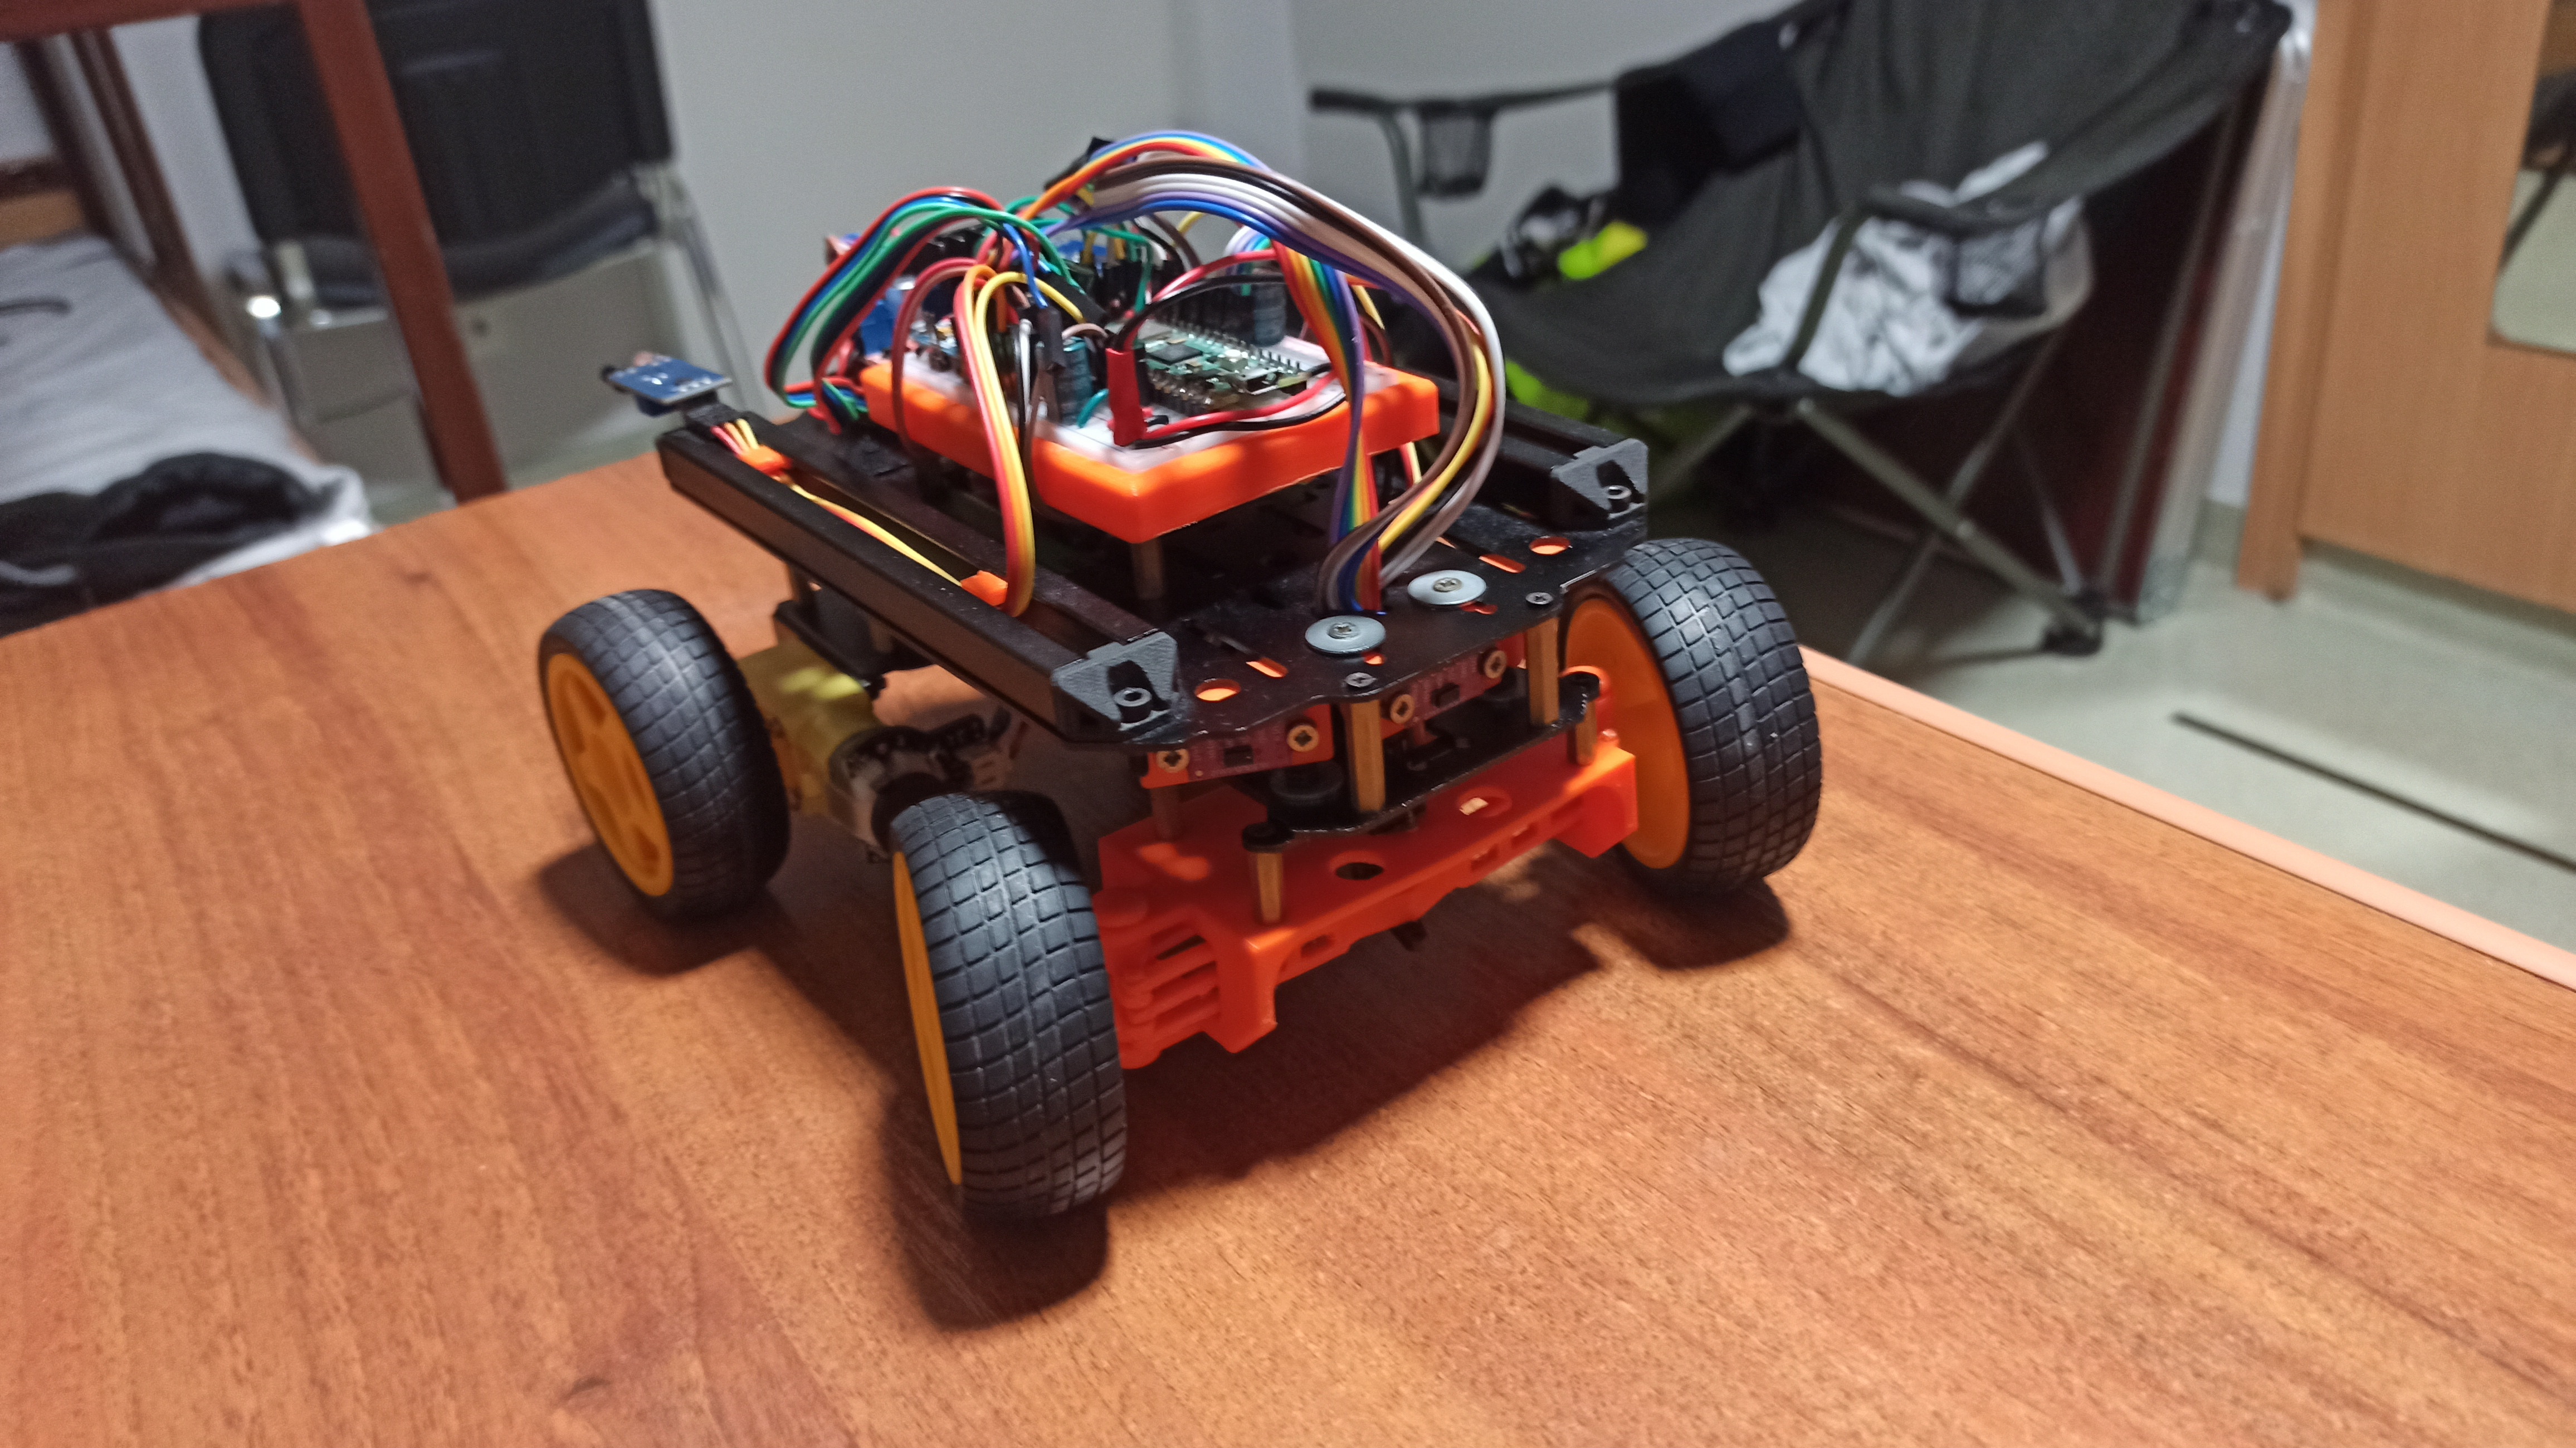
\includegraphics[width = 0.7\textwidth, trim = {800px, 400px, 1200px, 200px}, clip]{Breadboard_car.jpg}
            \caption{Model pojazdu z zainstalowaną płytą prototypową}
            \label{fig:breadboard_car}
        \end{figure}

        Po zamocowaniu płytki stykowej do prototypowej ramy, pojazd został poddany testom jednostkowym.
        Testy te polegały na sprawdzeniu działania wszystkich komponentów.
        Następnie, sprawdzono działanie podstawowych funkcji, typu jazda czy skręcanie.

        Podczas testowanie elementów pojedynczo, wszystko działało poprawnie.
        W czasie dłuższych testów, okazało się, że układ akcelerometru, potrafi zawiesić się w losowym momencie.
        Rozwiązaniem tego problemu, w tej wersji projektu, okazało się niemożliwe, ze względu na działanie płytki stykowej.
        Podczas jazdy, cały pojazd drżał, co powodowało, że niektóre piny nie stykały i układ akcelerometru, po spadku zasilania, blokował magistralę $I^2C$.

        Problematyczna okazała się linia $SDA$, protokołu $I^2C$.
        Rozwiązanie tego problemu było trudnym zadaniem.
        Szczególnie że bardzo ciężko było wykryć pierwotną przyczynę zawieszania się układu.
        Pierwszym rozwiązaniem problemu, było zastosowanie się do instrukcji z noty aplikacyjnej od Analog Devices o resetowaniu linii $I^2C$ \cite{application_note_I2C_AD}.
        Podobne rozwiązanie można znaleźć w dokumentacji do magistrali $I^2C$ \cite{I2C_manual_NXP} wydanej przez NXP.
        Niestety, zastosowane rozwiązanie nie przyniosło oczekiwanych rezultatów.

        Drugim rozwiązaniem sugerowanym przez oba dokumenty, w sytuacji kiedy nie udało się odblokować magistrali jest zresetowanie niedziałających (w domyśle wszystkich) układów.
        To rozwiązanie, mimo swojej skuteczności nie zostało wykorzystane.
        Autor skupił się na znalezieniu pierwotnej przyczyny problemu.

        Dodatkową zaletą wykonanie w pierwszej wersji projektu na płytce stykowej oraz losowego zawieszania się programu, było udoskonalenie funkcji odpowiedzialnych za kontrolę protokołu $I^2C$.
        W pierwszej wersji programu, komunikacja $I^2C$, blokowała pracę procesora.
        Rozwiązanie to sprawdzało się tak długo jak wszystko działało poprawnie.
        Jednak luźne połączenia ukazały, że to rozwiązanie jest niepraktyczne.
        W drugiej wersji programu, instrukcje odpowiedzialne za komunikację $I^2C$ zostały ograniczone \textit{timeoutem}.

        Ostateczną wersją prototypu jest płytka prototypowa, zlutowana na stałe.
        Zlutowanie układu na płytce, pozwoliło pozbyć się niektórych problemów, przykładowo blokowania się magistrali $I^2C$.
        Jednak złożenie zlutowanej wersji objawiło inne problemy, które ukrywała płytka stykowa.
        \begin{figure}[!ht]
            \centering
            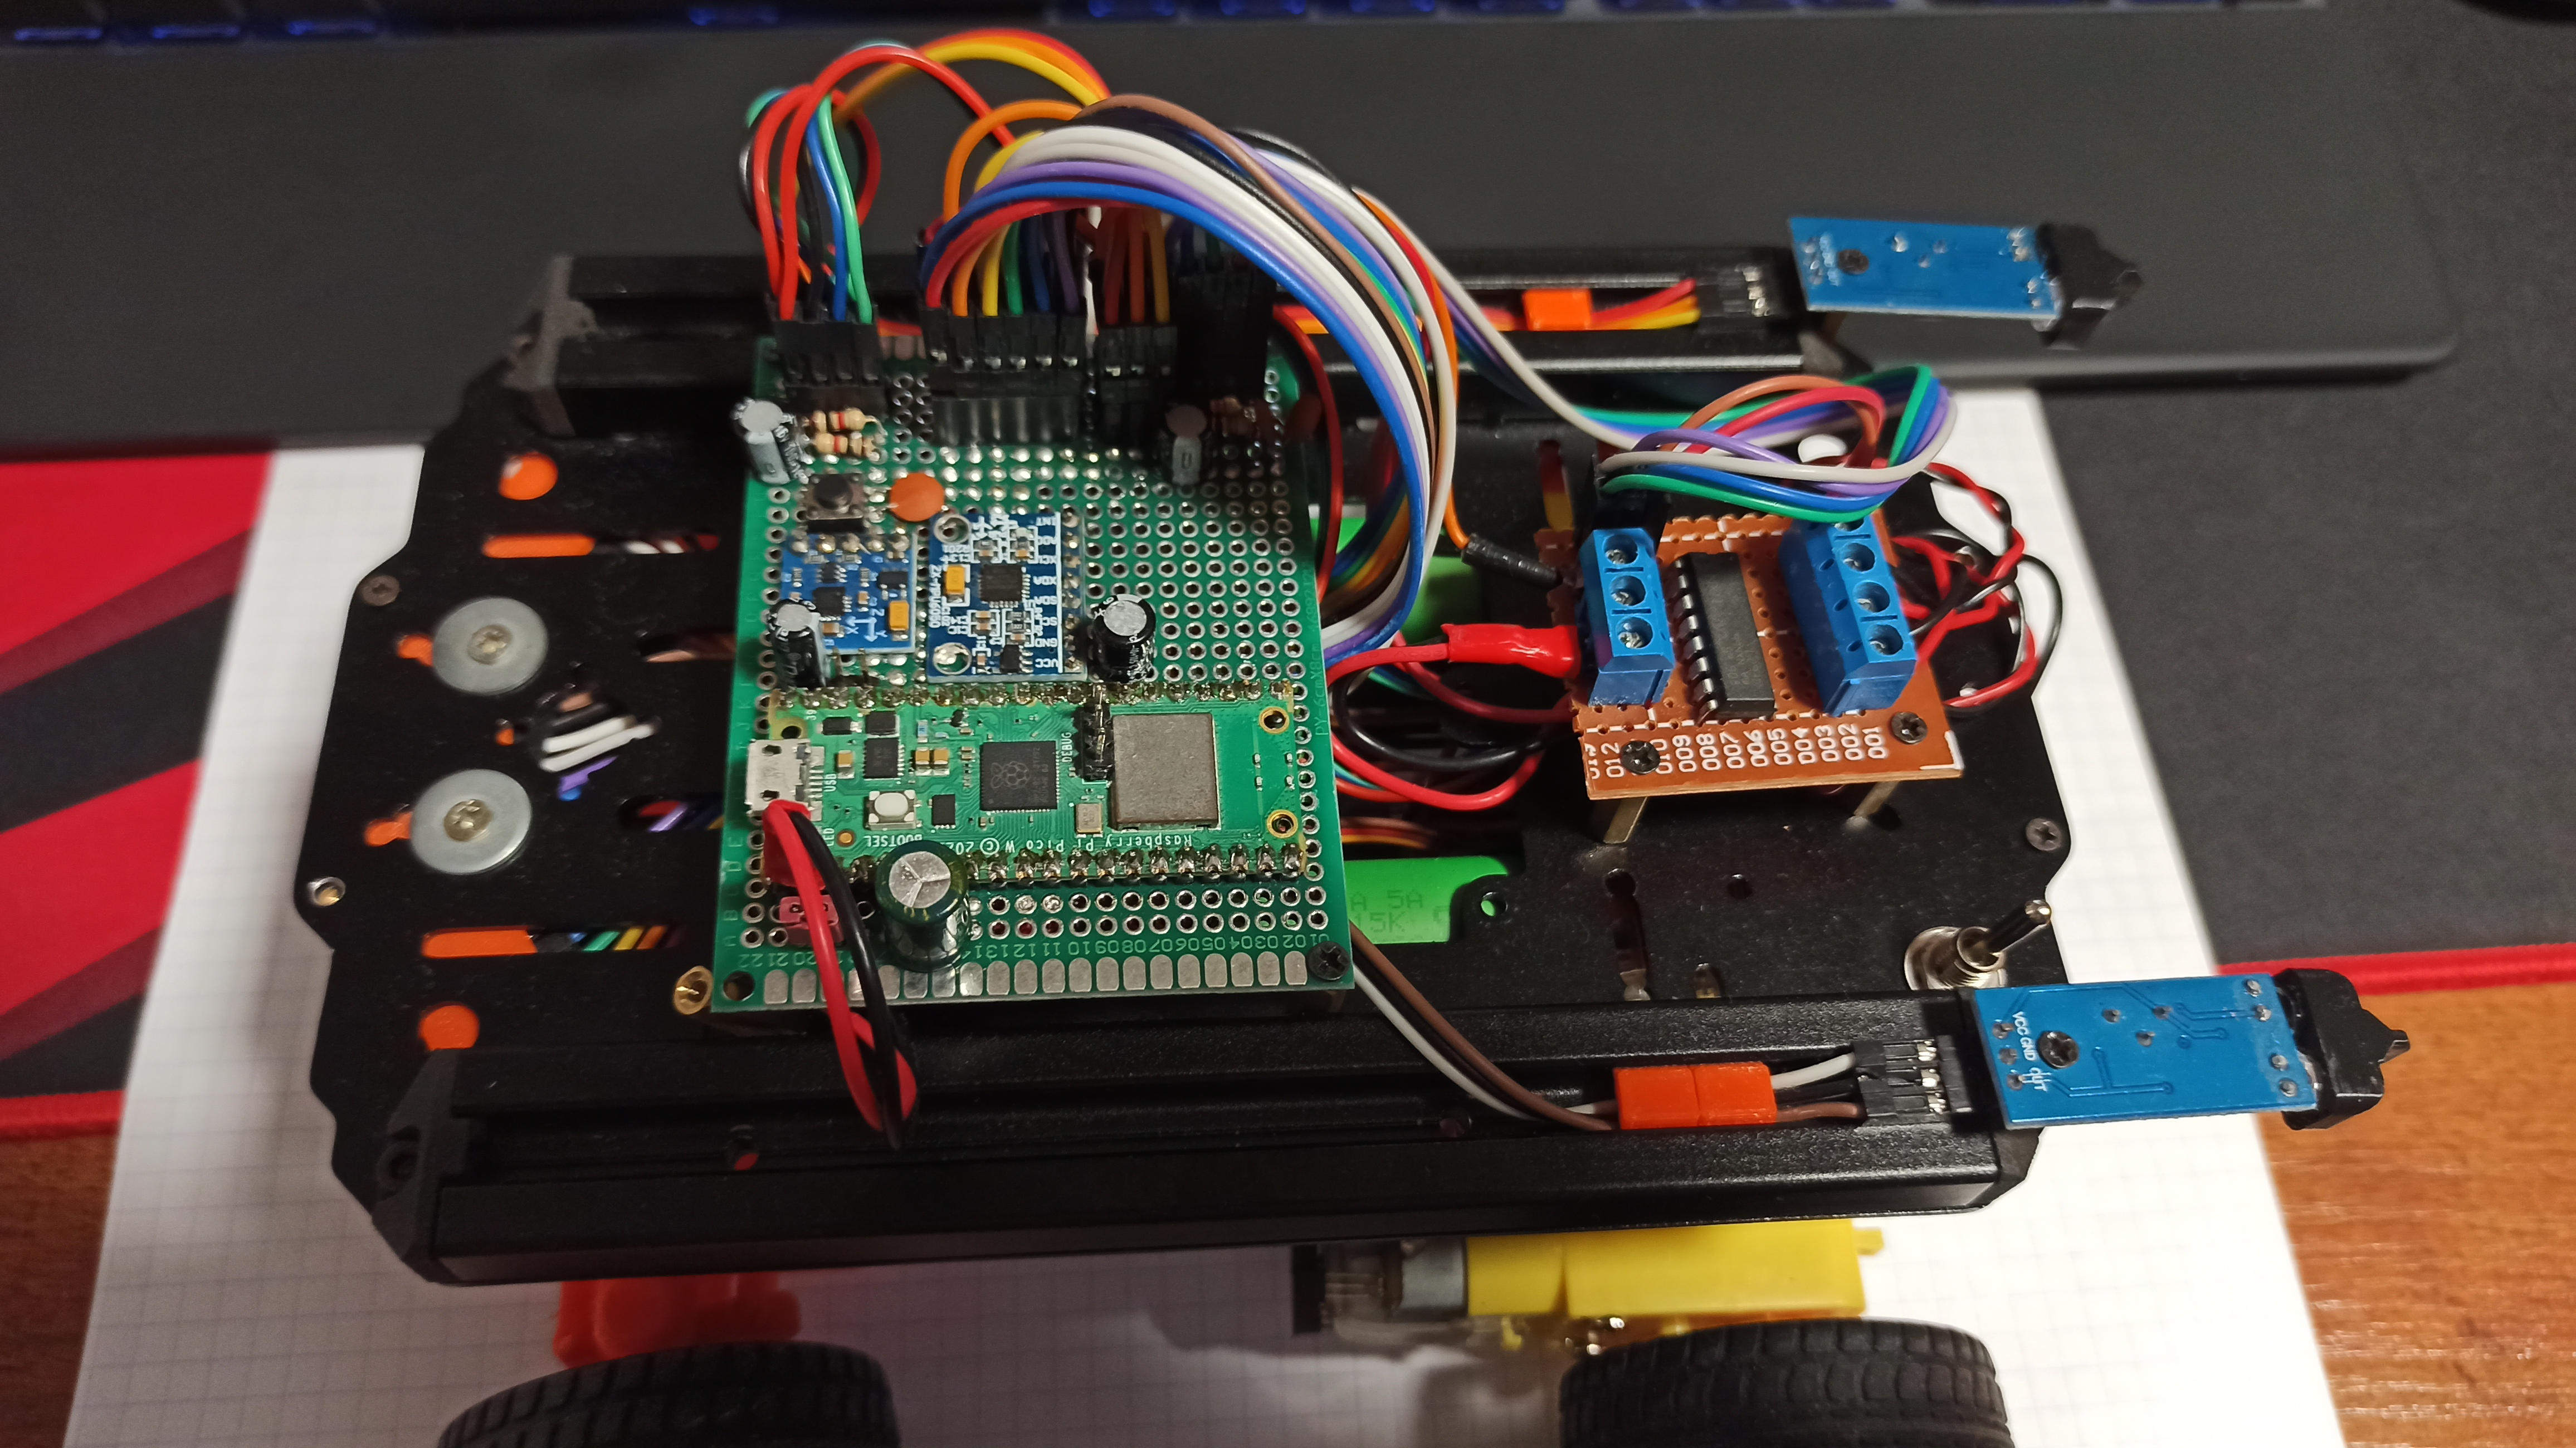
\includegraphics[width = 0.7\textwidth, trim = {500px, 300px, 300px, 200px}, clip]{Protoboard_car.jpg}
            \caption{Model pojazdu z zainstalowaną płytą prototypową}
            \label{fig:protoboard_car}
        \end{figure}

        Największym problemem, który pojawił się po zlutowaniu prototypu, było losowe resetowanie się RB Pi Pico (Raspberry Pi Pico).
        Znalezienie przyczyny tego problemu okazało się trudne.
        Problem występował czasami zarówno po podłączeniu zewnętrznego zasilacza jak i pracy na akumulatorach.
        Po testach okazało, się że sytuacja ta występuje tylko wtedy, gdy pracują silniki oraz podłączone są enkodery.
        Po odłączeniu wyjść sygnałowych enkoderów, kłopot z resetowaniem się układu zniknął.
        W celu upewnienia, się że przyczyną są uszkodzone enkodery, w szereg z wyjściem sygnałowym został podłączony rezystor o rezystancji $R =1k\Omega$.
        Po podłączeniu rezystora, problem z resetowaniem się układu zniknął na kilka dni.
        Po czym powrócił. Szukając problemów w okolicy silników, zostało zmienione zasilanie silników na niezależne od reszty układu.
        Uruchomienie silników, z zasilaniem niezależnym natychmiast zresetowało procesor.
        Kolejną próbą była zmiana mostka H na inny. Wymiana tego układu również nie pomogła.
        W między czasie podczas składania prototypu, uszkodzeniu uległ jeden z układów ToF.
        Po wymianie uszkodzonego układu, problem z resetowaniem się RB Pi Pico nie zniknął.
        Ostatnim pomysłem co mogło zostać uszkodzone, była sama malinka, jednak jej wymiana również nie pomogła.
        Ostatecznie, rozwiązaniem okazało się dołożenie dużej roznoszonej pojemności (około $500\mu F$) na całej płytce.

        Kolejnym problemem, na który natrafił autor, były oscylacje na liniach przerwań od czujników obiektów zamontowanych na tyle pojazdu.
        Oscylacje te, nie pozwalały na poruszanie się do tyłu, ponieważ czujniki w losowych momentach zgłaszały obiekt i zatrzymywały silniki.
        Rozwiązaniem tego problemu było zastosowanie filtru RC, który niweluje drgania.



    \subsection{Automatyzacja praca}
        Automatyzacja pracy jest niezwykle ważnym zadaniem w momencie, testowania podstawowych funkcji.
        Oczywiście, każdą funkcję można wywołać ręcznie, jednak podczas testów, kiedy wielokrotnie wykonywane są podobne funkcje, automatyzacja staje się obowiązkowa.

        Aby wykonać to zadanie, w języku Python został napisany skrypt, który pozwala na dwustronną komunikację za pomocą protokołu $UDP$.
        Dodatkowo, program pozwala na interpretację plików, napisanych specjalnie dla tego układu.
        Poniżej przedstawiono listing \eqref{list:self_test.s} programu do testowania podstawowych działań pojazdu.

        \lstinputlisting[style=asm, caption={Test pojazdu}, label = list:self_test.s]{Listing/self_test.s}

        \subsubsection{Interpreter własnego języka}
            Przedstawiony w listingu \ref{list:self_test.s} program jest interpretowanym przez skrypt napisany w pythonie.
            Jego zadaniem jest stokenizowanie instrukcji, wyznaczanie adresów skoków oraz stworzenie słownika z zmiennymi.
            Następnie, program przechodzi do wykonywania instrukcji zapisanych w pliku.
            Powyższy język posiada tylko kilka prostych słów kluczowych przedstawionych w tabeli \ref{table:keywords}.
            Pozostałe instrukcje po sformatowaniu wysyłane są do malinki.

            \begin{table}[!ht]
                \centering
                \caption{Lista słów kluczowych do mini języka}
                \begin{tabularx}{0.8\textwidth}{|c|c|C|}\hline
                    Nr. & Instrukcja & Opis \\\hline
                     1. & jump $etykieta$ & Skok do $etykiety$ \\\hline
                     2. & end & Koniec programu lub funkcji \\\hline
                     3. & print $zmienna/napis$ & Wypisanie wartości zmiennej lub napisu\\\hline
       \centerY{2}{ 5.} & \centerY{2}{if $warunek$} & Instrukcja warunkowa, w przypadku nie spełnienia pomija następną instrukcję\\\hline
       \centerY{2}{ 7.} & \centerY{2}{$etykieta$\textbf{:}} & Etykieta funkcji, koniecznie zakończona znakiem ,,:''\\\hline
       \centerY{4}{ 9.} & \centerY{4}{$\$zmienna$} & Odwołanie do zmiennej w przypadku instrukcji wysłanych. Podczas formatowania instrukcje, $\$zmienna$ zostaje podmieniona na wartość\\\hline
       \centerY{2}{10.} & \centerY{2}{$zmienna$ = \textit{wartość}} & Przypisanie wartości do zmiennej. Pozwala na wykonywanie operacji matematycznych\\\hline
                \end{tabularx}
                \label{table:keywords}
            \end{table}

            Wszystkie pozostałe instrukcje, które nie są zdefiniowane w tabeli, wysyłane są bezpośrednio do mikrokontroler.
            Natomiast w przypadku, kiedy instrukcja zostaje odnaleziona, ale zawiera błąd składniowy, program wyświetla błąd i przerwa działanie.
            Przykład takiej sytuacji przedstawiono na rysunku \ref{fig:interpreter}.

            \begin{figure}[!ht]
                \centering
                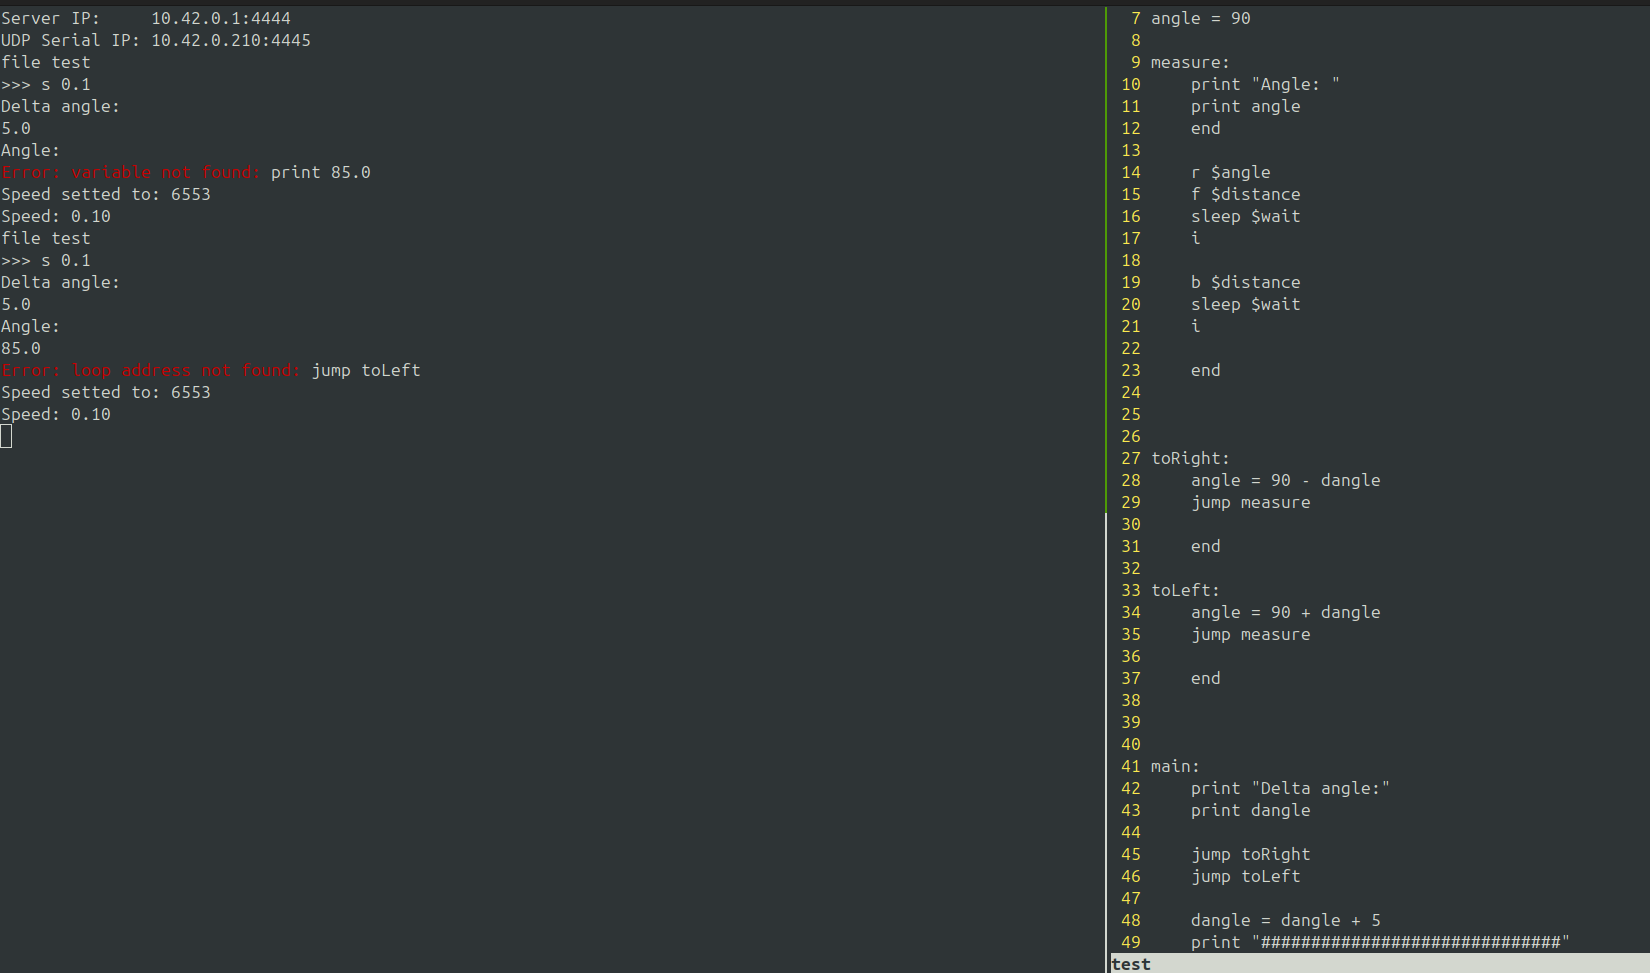
\includegraphics[width = 0.7\textwidth]{Terminal_program_testowy.png}
                \caption{Program zawierający celowe błędy}
                \label{fig:interpreter}
            \end{figure}

            W przypadku, kiedy program pracuje poprawnie, instrukcje wypisywane są równolegle z wiadomościami odebranymi od samochodu.
            Rozkazy wysyłane do mikrokontrolera, są poprzedzone łańcuchem znaków ,,$>>>$''.
            Natomiast instrukcja wynik instrukcji $print$ jest identyczny z tym, co zwraca mikrokontroler.
            Podczas testowania programy, program zdążył wysłać kilka instrukcji do raspberry dlatego po zgłoszeniu błedy widnieją widnieje kilka odebranych instrukcji.